\documentclass[14pt, a4paper]{article}
\usepackage{graphicx} % Required for inserting images

\usepackage[utf8]{inputenc}
\usepackage{amsmath}
\usepackage{amssymb}
\DeclareMathSymbol{\invques}{\mathord}{operators}{`>}
\DeclareUnicodeCharacter{00BF}{\tmquestiondown}
\DeclareRobustCommand{\tmquestiondown}{%
  \ifmmode\invques\else\textquestiondown\fi
}
\usepackage[portuges]{babel}%Babel -- irá activar automaticamente as regras apropriadas de hifenização para a língua todo o
                                   %-- o texto gerado é automaticamente traduzido para Português.
                                   %  Por exemplo, “chapter” irá passar a “capítulo”, “table of contents” a “conteúdo”.
                                   % portuges -- específica para o Português.
\usepackage[utf8]{inputenc} % define o encoding usado texto fonte (input)--usual "utf8" ou "latin1
\usepackage{parcolumns}

\usepackage{graphicx} %permite incluir graficos, tabelas, figuras
\usepackage{url} % para utilizar o comando \url{}
\usepackage{enumerate} %permite escolher, nas listas enumeradas, se os iems sao marcados com letras ou numeros-romanos em vez de numeracao normal

%\usepackage{apalike} % gerar biliografia no estilo 'named' (apalike)

\usepackage{color} % Para escrever em cores
\usepackage{multirow} %tabelas com multilinhas
\usepackage{array} %formatação especial de tabelas em array
\usepackage[pdftex]{hyperref} % transformar as referências internas do seu documento em hiper-ligações.
\usepackage{listings}
\usepackage{xcolor}
\definecolor{codegreen}{rgb}{0,0.6,0}
\definecolor{codegray}{rgb}{0.5,0.5,0.5}
\definecolor{codepurple}{rgb}{0.58,0,0.82}
\definecolor{backcolour}{rgb}{0.95,0.95,0.92}

\lstdefinestyle{mystyle}{
    backgroundcolor=\color{backcolour},   
    commentstyle=\color{codegreen},
    keywordstyle=\color{magenta},
    numberstyle=\tiny\color{codegray},
    stringstyle=\color{codepurple},
    basicstyle=\ttfamily\footnotesize,
    breakatwhitespace=false,         
    breaklines=true,                 
    captionpos=b,                    
    keepspaces=true,                 
    numbers=left,                    
    numbersep=5pt,                  
    showspaces=false,                
    showstringspaces=false,
    showtabs=false,                  
    tabsize=2
}

\lstset{style=mystyle}

%Exemplos de fontes -- nao e vulgar mudar o tipo de fonte
%\usepackage{tgbonum} % Fonte de letra: TEX Gyre Bonum
%\usepackage{lmodern} % Fonte de letra: Latin Modern Sans Serif
%\usepackage{helvet}  % Fonte de letra: Helvetica
%\usepackage{charter} % Fonte de letra:Charter

\definecolor{saddlebrown}{rgb}{0.55, 0.27, 0.07} % para definir uma nova cor, neste caso 'saddlebrown'

\usepackage{listings}  % para utilizar blocos de texto verbatim no estilo 'listings'
%paramerização mais vulgar dos blocos LISTING - GENERAL
\lstset{
	basicstyle=\small, %o tamanho das fontes que são usadas para o código
	numbers=left, % onde colocar a numeração da linha
	numberstyle=\tiny, %o tamanho das fontes que são usadas para a numeração da linha
	numbersep=5pt, %distancia entre a numeração da linha e o codigo
	breaklines=true, %define quebra automática de linha
    frame=tB,  % caixa a volta do codigo
	mathescape=true, %habilita o modo matemático
	escapeinside={(*@}{@*)} % se escrever isto  aceita tudo o que esta dentro das marcas e nao altera
}
%
%\lstset{ %
%	language=Java,							% choose the language of the code
%	basicstyle=\ttfamily\footnotesize,		% the size of the fonts that are used for the code
%	keywordstyle=\bfseries,					% set the keyword style
%	%numbers=left,							% where to put the line-numbers
%	numberstyle=\scriptsize,				% the size of the fonts that are used for the line-numbers
%	stepnumber=2,							% the step between two line-numbers. If it's 1 each line
%											% will be numbered
%	numbersep=5pt,							% how far the line-numbers are from the code
%	backgroundcolor=\color{white},			% choose the background color. You must add \usepackage{color}
%	showspaces=false,						% show spaces adding particular underscores
%	showstringspaces=false,					% underline spaces within strings
%	showtabs=false,							% show tabs within strings adding particular underscores
%	frame=none,								% adds a frame around the code
%	%abovecaptionskip=-.8em,
%	%belowcaptionskip=.7em,
%	tabsize=2,								% sets default tabsize to 2 spaces
%	captionpos=b,							% sets the caption-position to bottom
%	breaklines=true,						% sets automatic line breaking
%	breakatwhitespace=false,				% sets if automatic breaks should only happen at whitespace
%	title=\lstname,							% show the filename of files included with \lstinputlisting;
%											% also try caption instead of title
%	escapeinside={\%*}{*)},					% if you want to add a comment within your code
%	morekeywords={*,...}					% if you want to add more keywords to the set
%}

\usepackage{xspace} % deteta se a seguir a palavra tem uma palavra ou um sinal de pontuaçao se tiver uma palavra da espaço, se for um sinal de pontuaçao nao da espaço

\parindent=2pt %espaço a deixar para fazer a  indentação da primeira linha após um parágrafo
\parskip=4pt % espaço entre o parágrafo e o texto anterior

\setlength{\oddsidemargin}{-1cm} %espaço entre o texto e a margem
\setlength{\textwidth}{18cm} %Comprimento do texto na pagina
\setlength{\headsep}{-1cm} %espaço entre o texto e o cabeçalho
\setlength{\textheight}{23cm} %altura do texto na pagina

% comando '\def' usado para definir abreviatura (macros)
% o primeiro argumento é o nome do novo comando e o segundo entre chavetas é o texto original, ou sequência de controle, para que expande
\def\darius{\textsf{Darius}\xspace}
\def\antlr{\texttt{AnTLR}\xspace}
\def\titulo#1{\section{#1}}    %no corpo do documento usa-se na forma '\titulo{MEU TITULO}'
\def\super#1{{\em Supervisor: #1}\\ }
\def\area#1{{\em \'{A}rea: #1}\\[0.2cm]}
\def\resumo{\underline{Resumo}:\\ }
\def\e#1{\emph{#1}}


\title{Computação Gráfica (3º ano de LCC)\\
       \textbf{Trabalho Prático (Fase 2) — Grupo 1}\\ Relatório de Desenvolvimento}
\author{ Bruno Dias da Gião  (A96544) 
    \and Bruno Miguel Fernandes Araújo (A97509)
    \and João Luís da Cruz Pereira (A95375)}
\date{\today} %data

\begin{document}

\begin{titlepage}
\maketitle
\end{titlepage}

\tableofcontents
\listoffigures
\newpage
\section{Introdução} \label{sec:intro}

Este relatório serve como um apoio ao trabalho ,tem explicações sobre os raciocínios usados na segunda fase do projeto da unidade curricular Computação Gráfica.

Nesta fase apenas o engine foi modificado, sendo que foi necessário implementar o uso de transfomações sobre as figuras.

Tivemos de desenvolver um ficheiro \textit{XML} que através da leitura pelo engine , representará o Sistema Solar (ficheiro Demo).


\subsection{Estrutura do Relatório}
\begin{itemize}

\item \S\ref{sec:engine} - Nesta fase, passaremos a detalhar as classes de transformações
geométricas(\ref{subsec:classes}), a leitura do ficheiro XML(\ref{subsec:XML}) e
as gerações agrupadas de transformações e modelos(\ref{subsec:gera}).

\item \S\ref{sec:demo} - Explicação do desenvolvimento do ficheiro XML Demo.

\item \S\ref{sec:conclusion} - Conclusão e trabalho futuro.

\item \S\ref{sec:resultado} - Imagens tiradas dos modelos gerados a partir dos ficheiros \textit{XML} dos testes e da demo do Sistema Solar.
\end{itemize}

\section{\textit{Engine}} \label{sec:engine}
Passaremos a explicar o trabalho relativo ao {\bf Motor de Gráficos} concebido na fase anterior:
\subsection{Classes de Transformações}\label{subsec:classes}
Tirando proveito do principio de polimorfismo e herança de Programação Orientada a Objetos temos uma
superclasse \textit{\textbf{transform}}. que encapsula as classes \textit{\textbf{rotate}},
\textit{\textbf{scale}},\textit{\textbf{translate}}, identificadas por um selecionador do tipo,
para debug, com valores \verb|TRANS_ROT|, \verb|TRANS_SCA| e \verb|TRANS_TRA|, respetivamente.\\
Ora, cada subclasse contém variáveis privadas de transformação, construtores e um método que se
sobrepõe a um método da superclasse que invoca as funções respetivas de transformação da API do OpenGL,
como podemos ver nas seguintes definições:
\begin{lstlisting}[language=c++]
transform::transform(int t,float xx, float yy, float zz)
{this->a=0.f,this->type = t,this->x=xx,this->y=yy,this->z=zz;}
transform::transform(int t,float aa,float xx, float yy, float zz)
{this->a=aa,this->type = t,this->x=xx,this->y=yy,this->z=zz;}
void transform::do_transformation(){}
int transform::get_type(){return this->type;}
float transform::get_angle(){return this->a;}
float transform::get_x(){return this->x;}
float transform::get_y(){return this->y;}
float transform::get_z(){return this->z;}

rotate::rotate(float a,float xx, float yy, float zz)
	: transform(TRANS_ROT, a, xx, yy, zz){}
void rotate::do_transformation()
{glRotatef(this->get_angle(),this->get_x(),this->get_y(),this->get_z());}

scale::scale(float xx, float yy, float zz)
	:transform(TRANS_SCA, xx, yy, zz){}
void scale::do_transformation()
{glScalef(this->get_x(),this->get_y(),this->get_z());}

translate::translate(float xx, float yy, float zz)
	: transform(TRANS_TRA, xx, yy, zz){}
void translate::do_transformation()
{glTranslatef(this->get_x(),this->get_y(),this->get_z());}

\end{lstlisting}
\subsection{Leitura do ficheiro de configuração}\label{subsec:XML}
A estrutura do ficheiro de configuração é uma versão estendida do ficheiro de configuração da primeira
fase, tendo adicionado a interpretação de elementos \verb|transform| que pode conter $n\in\mathbb{N}$
transformações de tipo:$$t\in\{\verb|TRANS_ROT|,\verb|TRANS_SCA|,\verb|TRANS_TRA|\}$$.
Sendo assim, a sua leitura, ao contrário da primeira fase, passa a ser feita de forma recursiva seguindo
a seguinte implementação:
\begin{lstlisting}[language=c++]
void group_read(int cur_parent, int cur_g, XMLElement*gr,
               bool reading = false,
               int i=0)
{
	XMLElement*elem = !reading ? gr->FirstChildElement():
		gr->NextSiblingElement();
	if (cur_g == -1 || !elem)
		return;
    if (cur_parent > -1 && !reading) {
		for (int i=0; i<world.transformations.size(); i++) {
            struct trans copia;
            if (world.transformations[i].group == cur_parent) {
                copia.group = cur_g;
                copia.t = world.transformations[i].t;
                world.transformations.push_back(copia);
            }
        }
	}
	if (cur_g >= global)
		global = cur_g+1;
	if (!strcmp(elem->Name(),"models"))
		group_read_models(cur_parent, cur_g, elem);
	else if (!strcmp(elem->Name(), "transform"))
		group_read_transform(cur_parent, cur_g, elem);
	else if (!strcmp(elem->Name(), "group"))
		group_read(cur_g, global, elem,  false, i);
	group_read(cur_parent, cur_g, elem, true, i);
}
\end{lstlisting}
Todas as outras funcões invocadas por esta seguem o mesmo padrão recursivo de guardar o grupo ``pai''
e o grupo atual nos argumentos e ``iterar'' sobre o grupo sabendo essa informação, na sua essência,
sabendo se a ``iteração'' atual é a primeira ou não procuramos o primeiro filho ou o próximo irmão,
respetivamente, acabando quando este proximo elemento for nulo ou chegarmos a uma chamada recursiva onde
a raiz em si do ficheiro XML é o grupo atual.
\subsubsection{Agrupamento do Desenho de modelos e Aplicação de transformações}\label{subsec:gera}
De notar o segmento de código que itera sobre \verb|world.transformations| quando o pai atual não é a
raiz do ficheiro de configuração, este permite uma funcionalidade de extrema importância: a herança de
transformação dos grupos pais para os seus filhos.\\
Já o desenho das figuras tem uma pequena alteração, isto pois, com transformações o desenho de figuras
terá de ser segregado em grupos, sendo assim, iterando sobre o número de grupos, que é
computado de acordo com o maior valor atual do grupo na leitura recursiva, conseguimos comparar o nome associado a um conjunto de coordenadas com o nome associado à primitiva em si, o que permite verificar
se pertence ao grupo a ser trabalhado, como podemos ver no seguinte segmento de código:
\begin{lstlisting}[language=c++]
void drawfigs(void)
{
	int i, j, k, l, g;
    for (g=0; g<global; g++) {
		glPushMatrix();
		for (l=0;l<world.transformations.size();l++) /* trans*/
			if (world.transformations[l].group == g) {
				world.transformations[l].t->do_transformation();
            }
        for (k=0; k<world.primitives.size(); k++) {
            if (world.primitives[k].group == g) {
                for (i = 0; i<prims.size(); i++) {
                    if (!strcmp(prims[i].name, world.primitives[k].name)) {
		                glBegin(GL_TRIANGLES);
                        for (j=0; j<prims[i].coords.size();j++) {
                            glVertex3f(prims[i].coords[j].x,
                                   prims[i].coords[j].y,
                                   prims[i].coords[j].z);
                        }
		                glEnd();
                    }
                }
            }
        }
		glPopMatrix();
	}
}
\end{lstlisting}
De notar a forma como o código é completamente agnóstico ao tipo de transformações e ao tipo de
primitiva, verificando exclusivamente se pertence ao grupo estudado e quais sãos os valores das
coordenadas.

\section{Desenvolvimento da Demo} \label{sec:demo}
Para a representação do sistema solar, decidimos colocar cada planeta num grupo , cujo este terá como subgrupos as suas luas ou no caso de Júpiter, também o seu anel.

Usamos o mesmo ficheiro modelo da esfera para representar os planetas e as luas de forma a evitar ter de gerar e de ler diferentes ficheiros, assim apenas é necessário gerar um que será lido uma vez no engine.

Demos uso da figura extra que desenvolvemos na fase anterior , o torus, para criarmos o anel de Júpiter.

Para as diferenças de tamanho e de distância ao Sol dos planetas, usamos as transformações scale e translate , respetivamente.

Veremos então como exemplo o caso da Terra com a Lua:
\begin{lstlisting}[language=XML]
<group> 
     <transform>
         <translate x="80" y="0" z="80" />
         <scale x="0.4" y="0.4" z="0.4" />
     </transform>
              <models> 
                   <model file="sphere_10_20_20.3d" /> <!-- Terra -->
              </models>
              <group> 
                   <transform> 
                         <translate x="24" y="24" z="24" />
                         <scale x="0.1" y="0.1" z="0.1" />
                   </transform>
                         <models> 
                              <model file="sphere_10_20_20.3d" /> <!-- Lua -->
                         </models>
              </group>						
</group>
\end{lstlisting}

Como nesta fase foi nos indicado fazer uma representação inicial, não definimos nenhuma escala apropriada, nem foram colocadas todas as luas dos planetas.Apesar disto tivemos em conta os seus tamanhos para irmos de encontro com a realidade, ou seja se um planeta é mais pequeno que outro, este também o vai ser no nosso modelo.

\section{Conclusão} \label{sec:conclusion}

Efetuamos as alterações necessárias no nosso \textbf{motor} de gráficos para o mesmo ser capaz de, interpretar um ficheiro XML com diversos grupos, transformações e modelos, como pedido no enunciado do projeto. Elaboramos também um ficheiro XML para modelar uma simulação do sistema solar.

\subsection{Trabalho Futuro}
Para além do conteúdo requisito das fases ainda por realizar, temos certos objetivos pessoais que
gostavamos de realizar ao longo da elaboração do projeto, nomeadamente:
\begin{itemize}
    \item A implementação de $3$ tipos de câmaras que podem ser predefinidas no input XML e alteradas ao
    longo da execução do engine, particularmente, uma câmara explorador, uma câmara primeira pessoa e
    uma câmara terceira pessoa\footnote{ver Eve Online - \url{https://www.eveonline.com/}}.
    \item Otimização do \textbf{engine} atrav\'es do desenho das primitivas usando VBOs e VBOs com indexação.
    \item Criação de mais tipos de primitivas como, por exemplo, o teapot ou prismas.
\end{itemize}


\newpage
\section{Resultados} \label{sec:resultado}

Os resultados obtidos para cada teste fornecido e para um exemplo do torus.

\begin{figure}[ht]
\centering
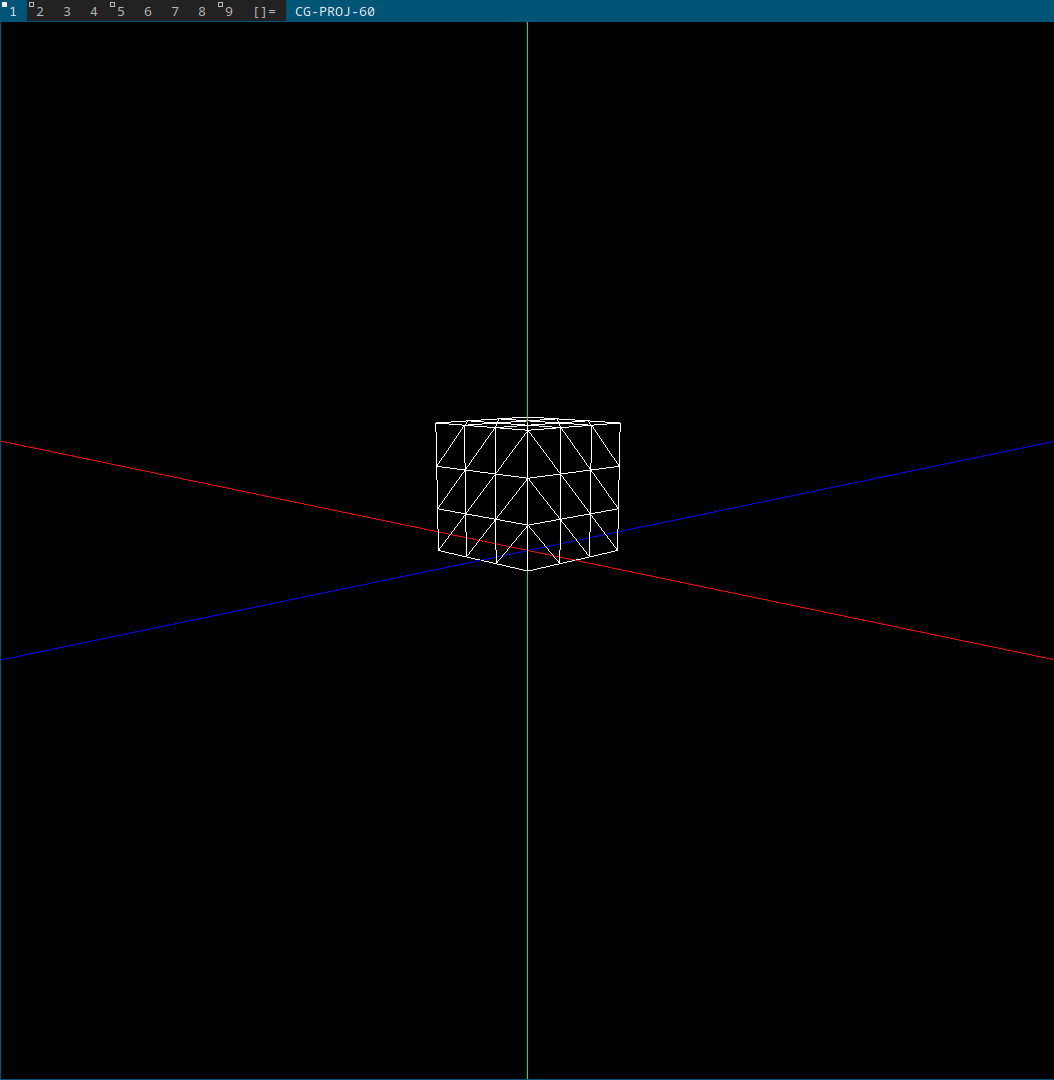
\includegraphics[width=0.5\textwidth]{images/1.png}
\caption{Teste 1}
\end{figure}

\begin{figure}[ht]
\centering
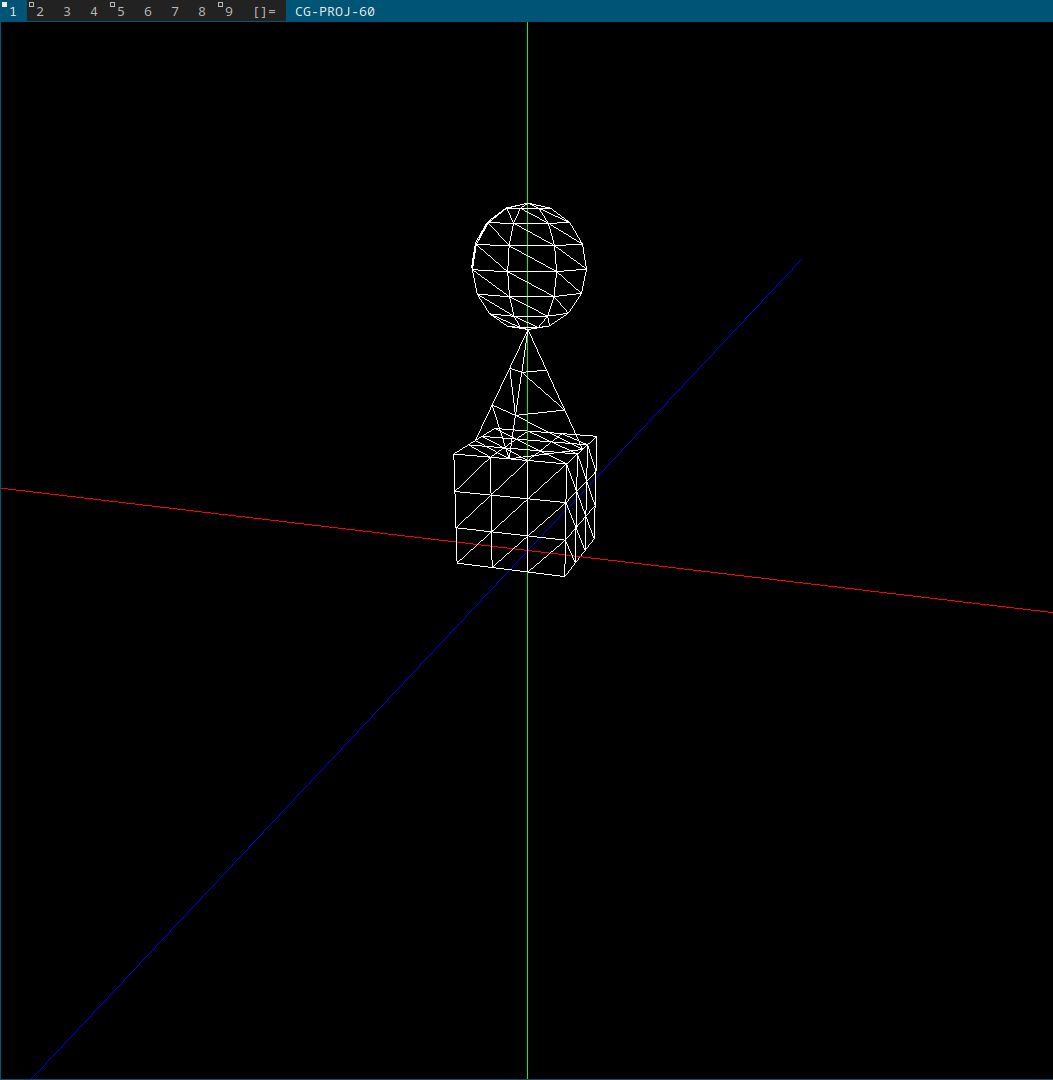
\includegraphics[width=0.5\textwidth]{images/2.png}
\caption{Teste 2}
\end{figure}

\begin{figure}[ht]
\centering
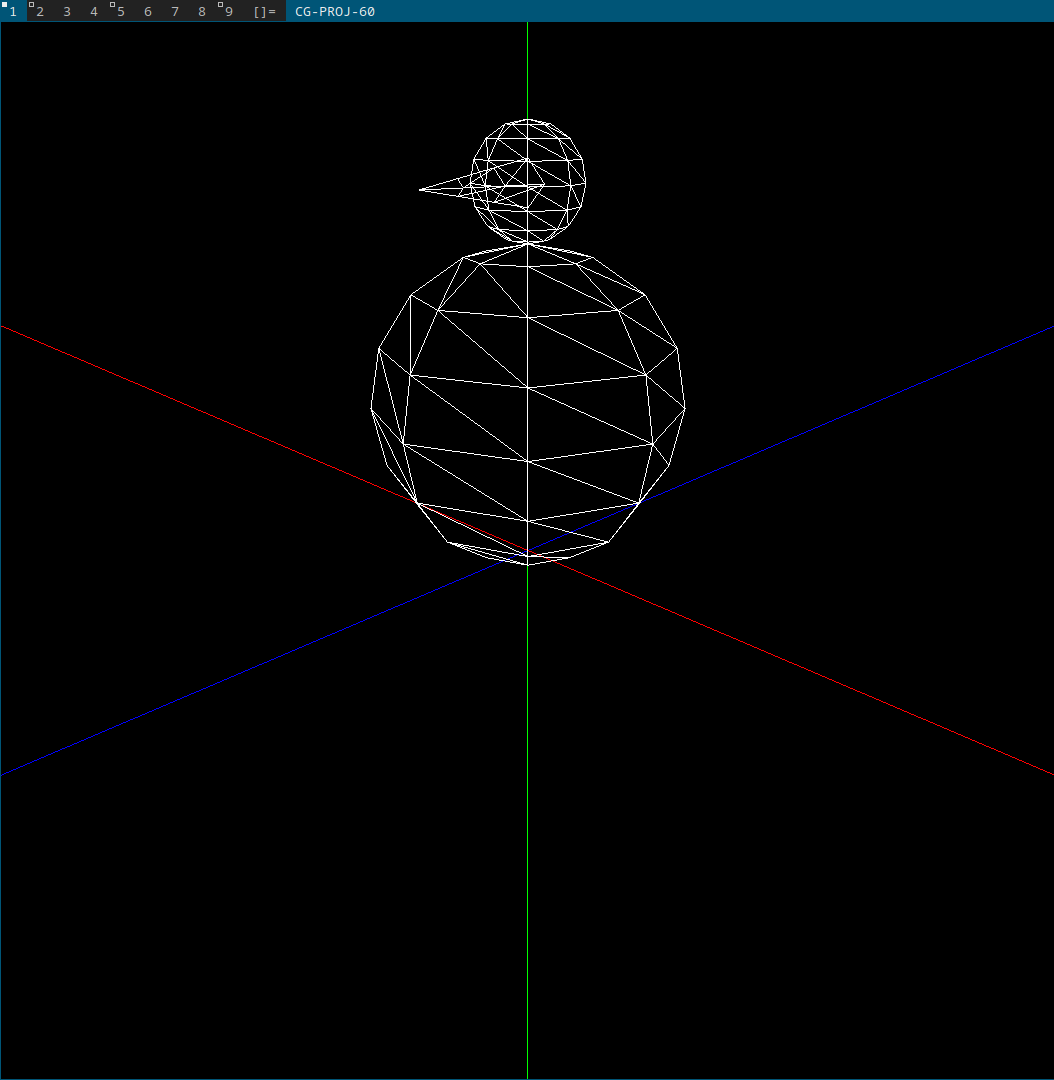
\includegraphics[width=0.5\textwidth]{images/3.png}
\caption{Teste 3}
\end{figure}

\begin{figure}[ht]
\centering
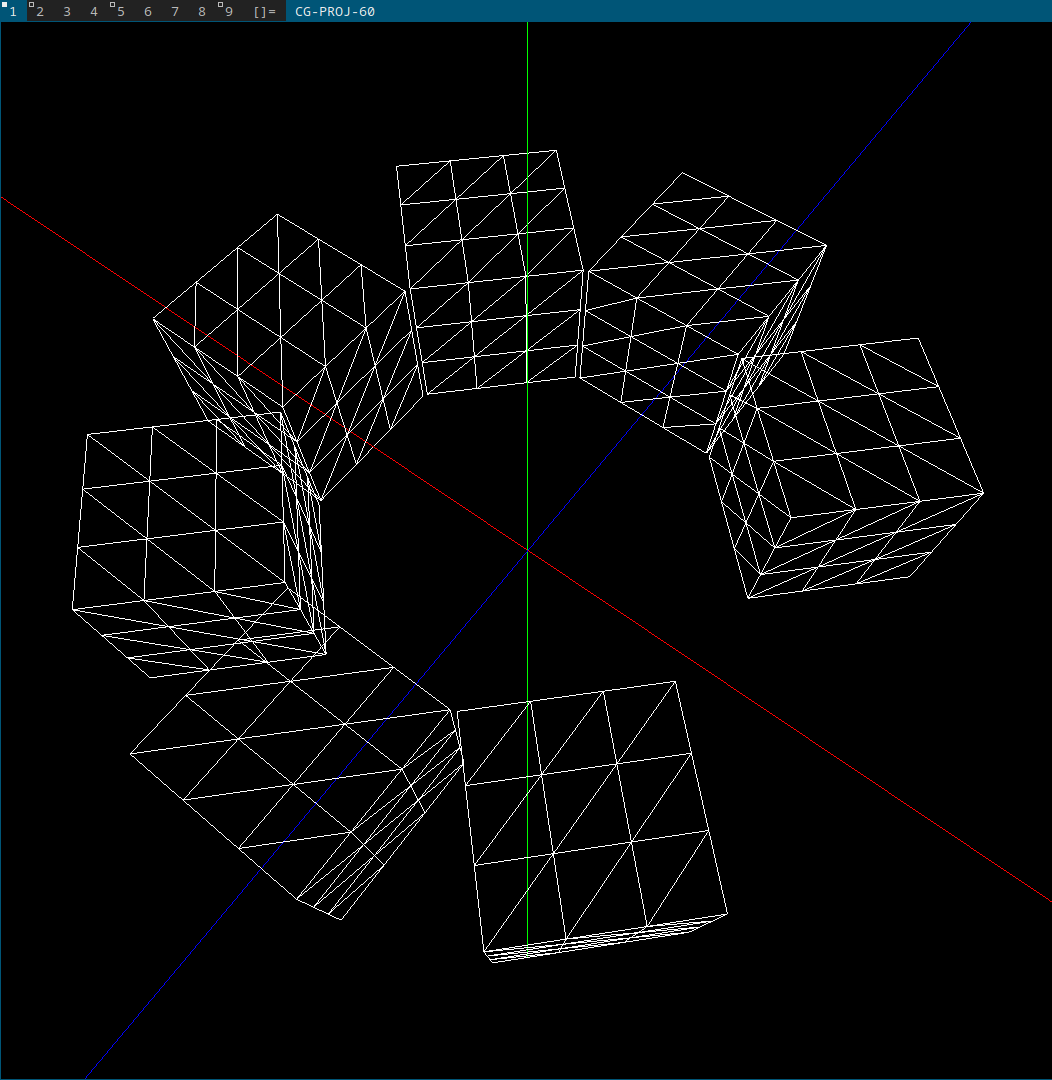
\includegraphics[width=0.5\textwidth]{images/4.png}
\caption{Teste 4}
\end{figure}

\begin{figure}[ht]
\centering
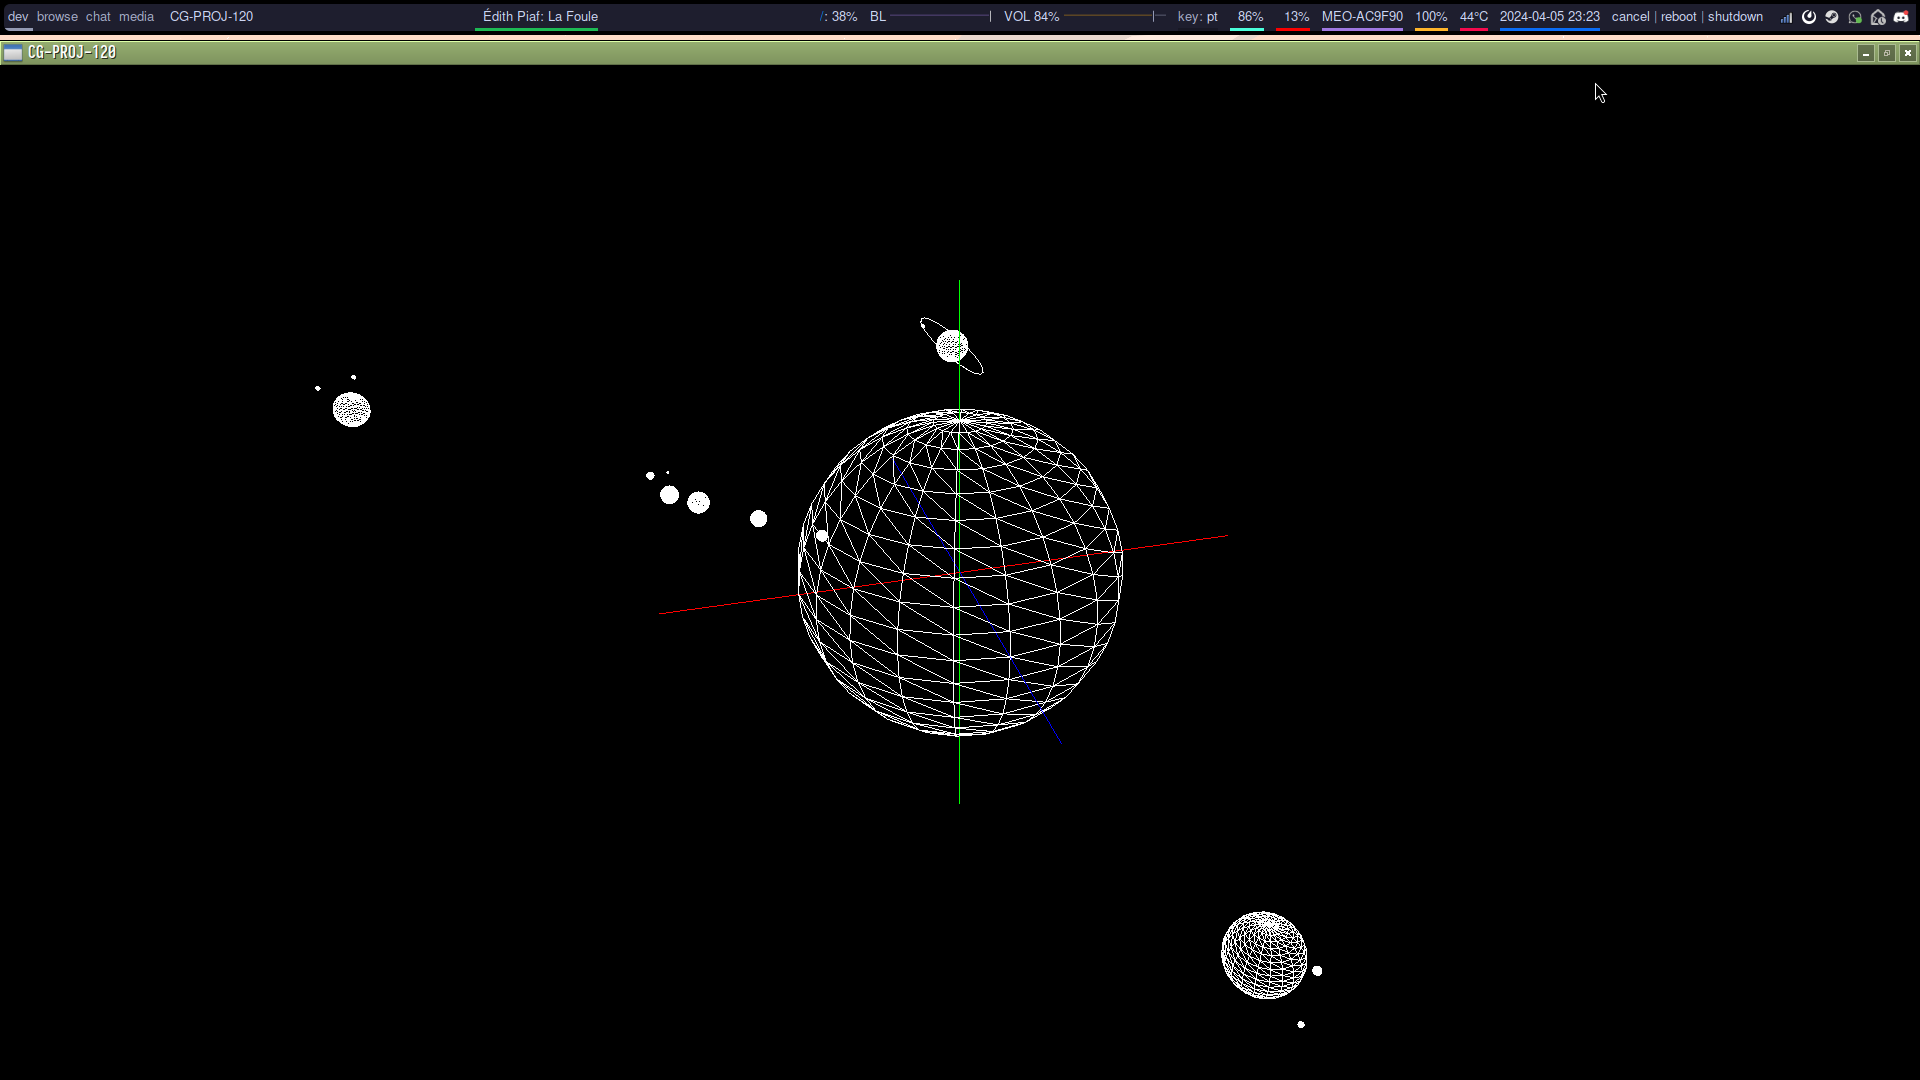
\includegraphics[width=0.5\textwidth]{images/5.png}
\caption{Sistema Solar}
\end{figure}

\end{document}
